%% Infografia_DCBI_2026.tex
%% Infografía de 2 páginas — Resultados del análisis de similitud DCBI 2026
%% Compilar: pdflatex Infografia_DCBI_2026.tex

\documentclass[9pt,a4paper]{article}
\usepackage[margin=0.55cm,top=0.50cm,bottom=0.50cm]{geometry}
\usepackage[utf8]{inputenc}
\usepackage[T1]{fontenc}
\usepackage[spanish,mexico]{babel}
\decimalpoint
\usepackage{lmodern}
\renewcommand{\familydefault}{\sfdefault}
\usepackage{microtype}
\usepackage{amsmath,amssymb}
\usepackage{graphicx}
\graphicspath{{../}}
\usepackage[table]{xcolor}
\usepackage{tcolorbox}
\tcbuselibrary{skins,breakable}
\usepackage{booktabs,array}

\pagestyle{empty}
\parindent=0pt
\parskip=0pt

%% ── Paleta UAM-A ───────────────────────────────────────────────────────────
\definecolor{uamred}{RGB}{200,45,35}
\definecolor{uamlightred}{RGB}{248,232,232}
\definecolor{uamblue}{RGB}{28,28,28}
\definecolor{uamgray}{RGB}{120,120,120}
\definecolor{uamlgray}{RGB}{243,243,243}
\definecolor{navy}{RGB}{21,61,132}
\definecolor{teal}{RGB}{0,131,143}
\definecolor{forest}{RGB}{46,125,50}
\definecolor{amber}{RGB}{160,108,0}
%% Licenciaturas
\definecolor{cInd}{RGB}{198,40,40}
\definecolor{cMec}{RGB}{55,71,79}
\definecolor{cFis}{RGB}{0,131,143}
\definecolor{cAmb}{RGB}{46,125,50}
\definecolor{cQui}{RGB}{85,139,47}
\definecolor{cCiv}{RGB}{191,54,12}
\definecolor{cCmp}{RGB}{21,101,192}
\definecolor{cElc}{RGB}{180,120,0}
\definecolor{cEle}{RGB}{106,27,154}
\definecolor{cMet}{RGB}{120,144,156}

%% ── Macros tipográficos ────────────────────────────────────────────────────
\newcommand{\BIGNUM}[1]{{\fontsize{26}{28}\selectfont\bfseries#1}}
\newcommand{\MEDNUM}[1]{{\fontsize{17}{19}\selectfont\bfseries#1}}
\newcommand{\LABEL}[1]{{\small\bfseries\color{uamblue}#1}}
\newcommand{\NOTE}[1]{{\footnotesize\color{uamgray}#1}}
\newcommand{\SECTHEAD}[1]{%
  {\footnotesize\bfseries\color{uamblue}\MakeUppercase{#1}}\par\vspace{2pt}}

%% ── Estilos tcolorbox ─────────────────────────────────────────────────────
\tcbset{
  hdr/.style={enhanced,sharp corners,colback=uamred,colframe=uamred,
    left=8pt,right=8pt,top=5pt,bottom=5pt,
    before skip=0pt,after skip=4pt},
  statcard/.style={enhanced,sharp corners,
    left=6pt,right=6pt,top=5pt,bottom=5pt,
    before skip=0pt,after skip=0pt},
  findcard/.style={enhanced,sharp corners,
    left=8pt,right=6pt,top=4pt,bottom=4pt,
    before skip=2pt,after skip=2pt},
  famcard/.style={enhanced,sharp corners,
    left=5pt,right=5pt,top=4pt,bottom=4pt,
    before skip=0pt,after skip=0pt},
  figbox/.style={enhanced,colback=white,colframe=uamlgray,
    sharp corners,top=3pt,bottom=3pt,left=3pt,right=3pt,
    before skip=0pt,after skip=0pt},
  grayband/.style={enhanced,colback=uamlgray,colframe=uamlgray,
    sharp corners,left=6pt,right=6pt,top=4pt,bottom=4pt,
    before skip=3pt,after skip=3pt},
  whitebox/.style={enhanced,colback=white,colframe=uamlgray,
    sharp corners,left=6pt,right=6pt,top=4pt,bottom=4pt,
    before skip=3pt,after skip=3pt}
}

\begin{document}

%%════════════════════════════════════════════════════════════════════════════
%% PÁGINA 1 — El corpus, el método y los resultados
%%════════════════════════════════════════════════════════════════════════════

%% ── Encabezado ─────────────────────────────────────────────────────────────
\begin{tcolorbox}[hdr]
\begin{minipage}[c]{0.079\linewidth}
  \includegraphics[width=\linewidth,trim={48bp 64bp 473bp 35bp},clip]%
    {/Users/nowhere/Claude_Projects/Personal/logo_UAM.png}
\end{minipage}\hfill
\begin{minipage}[c]{0.910\linewidth}
  {\fontsize{12.5}{14.5}\selectfont\bfseries\color{white}%
   ANÁLISIS DE SIMILITUD DE CONTENIDOS ENTRE PROGRAMAS DE UEA}\\[1pt]
  {\small\color{white!70!uamred}%
   Proceso de modificación curricular 2026 \;$\cdot$\;
   División de Ciencias Básicas e Ingeniería \;$\cdot$\; UAM-Azcapotzalco}
\end{minipage}
\end{tcolorbox}

%% ── Tres estadísticas clave ────────────────────────────────────────────────
\begin{minipage}[t]{0.315\linewidth}
\begin{tcolorbox}[statcard,colback=navy!10,colframe=navy!30]
\centering
\BIGNUM{\color{navy}626}\\[1pt]
\LABEL{programas de UEA en corpus}\\[1pt]
\NOTE{773 inventariados $\cdot$ excluye Tronco General}
\end{tcolorbox}
\end{minipage}\hfill
\begin{minipage}[t]{0.315\linewidth}
\begin{tcolorbox}[statcard,colback=teal!9,colframe=teal!30]
\centering
\BIGNUM{\color{teal}195{,}375}\\[1pt]
\LABEL{pares posibles evaluados}\\[1pt]
\NOTE{$\binom{626}{2}$ combinaciones de programas}
\end{tcolorbox}
\end{minipage}\hfill
\begin{minipage}[t]{0.315\linewidth}
\begin{tcolorbox}[statcard,colback=forest!9,colframe=forest!30]
\centering
\BIGNUM{\color{forest}1{,}505}\\[1pt]
\LABEL{re-evaluados semánticamente}\\[1pt]
\NOTE{por el LLM en 141\,s · \$0.24\,USD}
\end{tcolorbox}
\end{minipage}

\vspace{3pt}

%% ── Pipeline (texto en línea, sin cajas apiladas) ────────────────────────
\begin{tcolorbox}[grayband]
\SECTHEAD{pipeline híbrido de dos fases}
\centering
{\small\textbf{\color{navy}Texto UEA}}~%
$\xrightarrow{\;\text{\tiny TF-IDF bigramas, 8k dims}\;}$~%
{\small\textbf{\color{navy}Similitud coseno $626\!\times\!626$}}~%
$\xrightarrow{\;\text{\tiny umbral }s\geq0.20\;}$~%
{\small\textbf{\color{navy}1,505 pares candidatos}}~%
$\xrightarrow{\;\text{\tiny LLM re-evalúa}\;}$~%
{\small\textbf{\color{uamred}Matriz híbrida $626\!\times\!626$}}
\end{tcolorbox}

\vspace{3pt}

%% ── Heatmap media-máxima + resultados ──────────────────────────────────────
\begin{minipage}[t]{0.565\linewidth}
\begin{tcolorbox}[figbox]
{\footnotesize\bfseries\color{uamblue}Similitud media-máxima $\bar{s}(A,B)$ entre los 10 planes de estudio}\par\vspace{2pt}
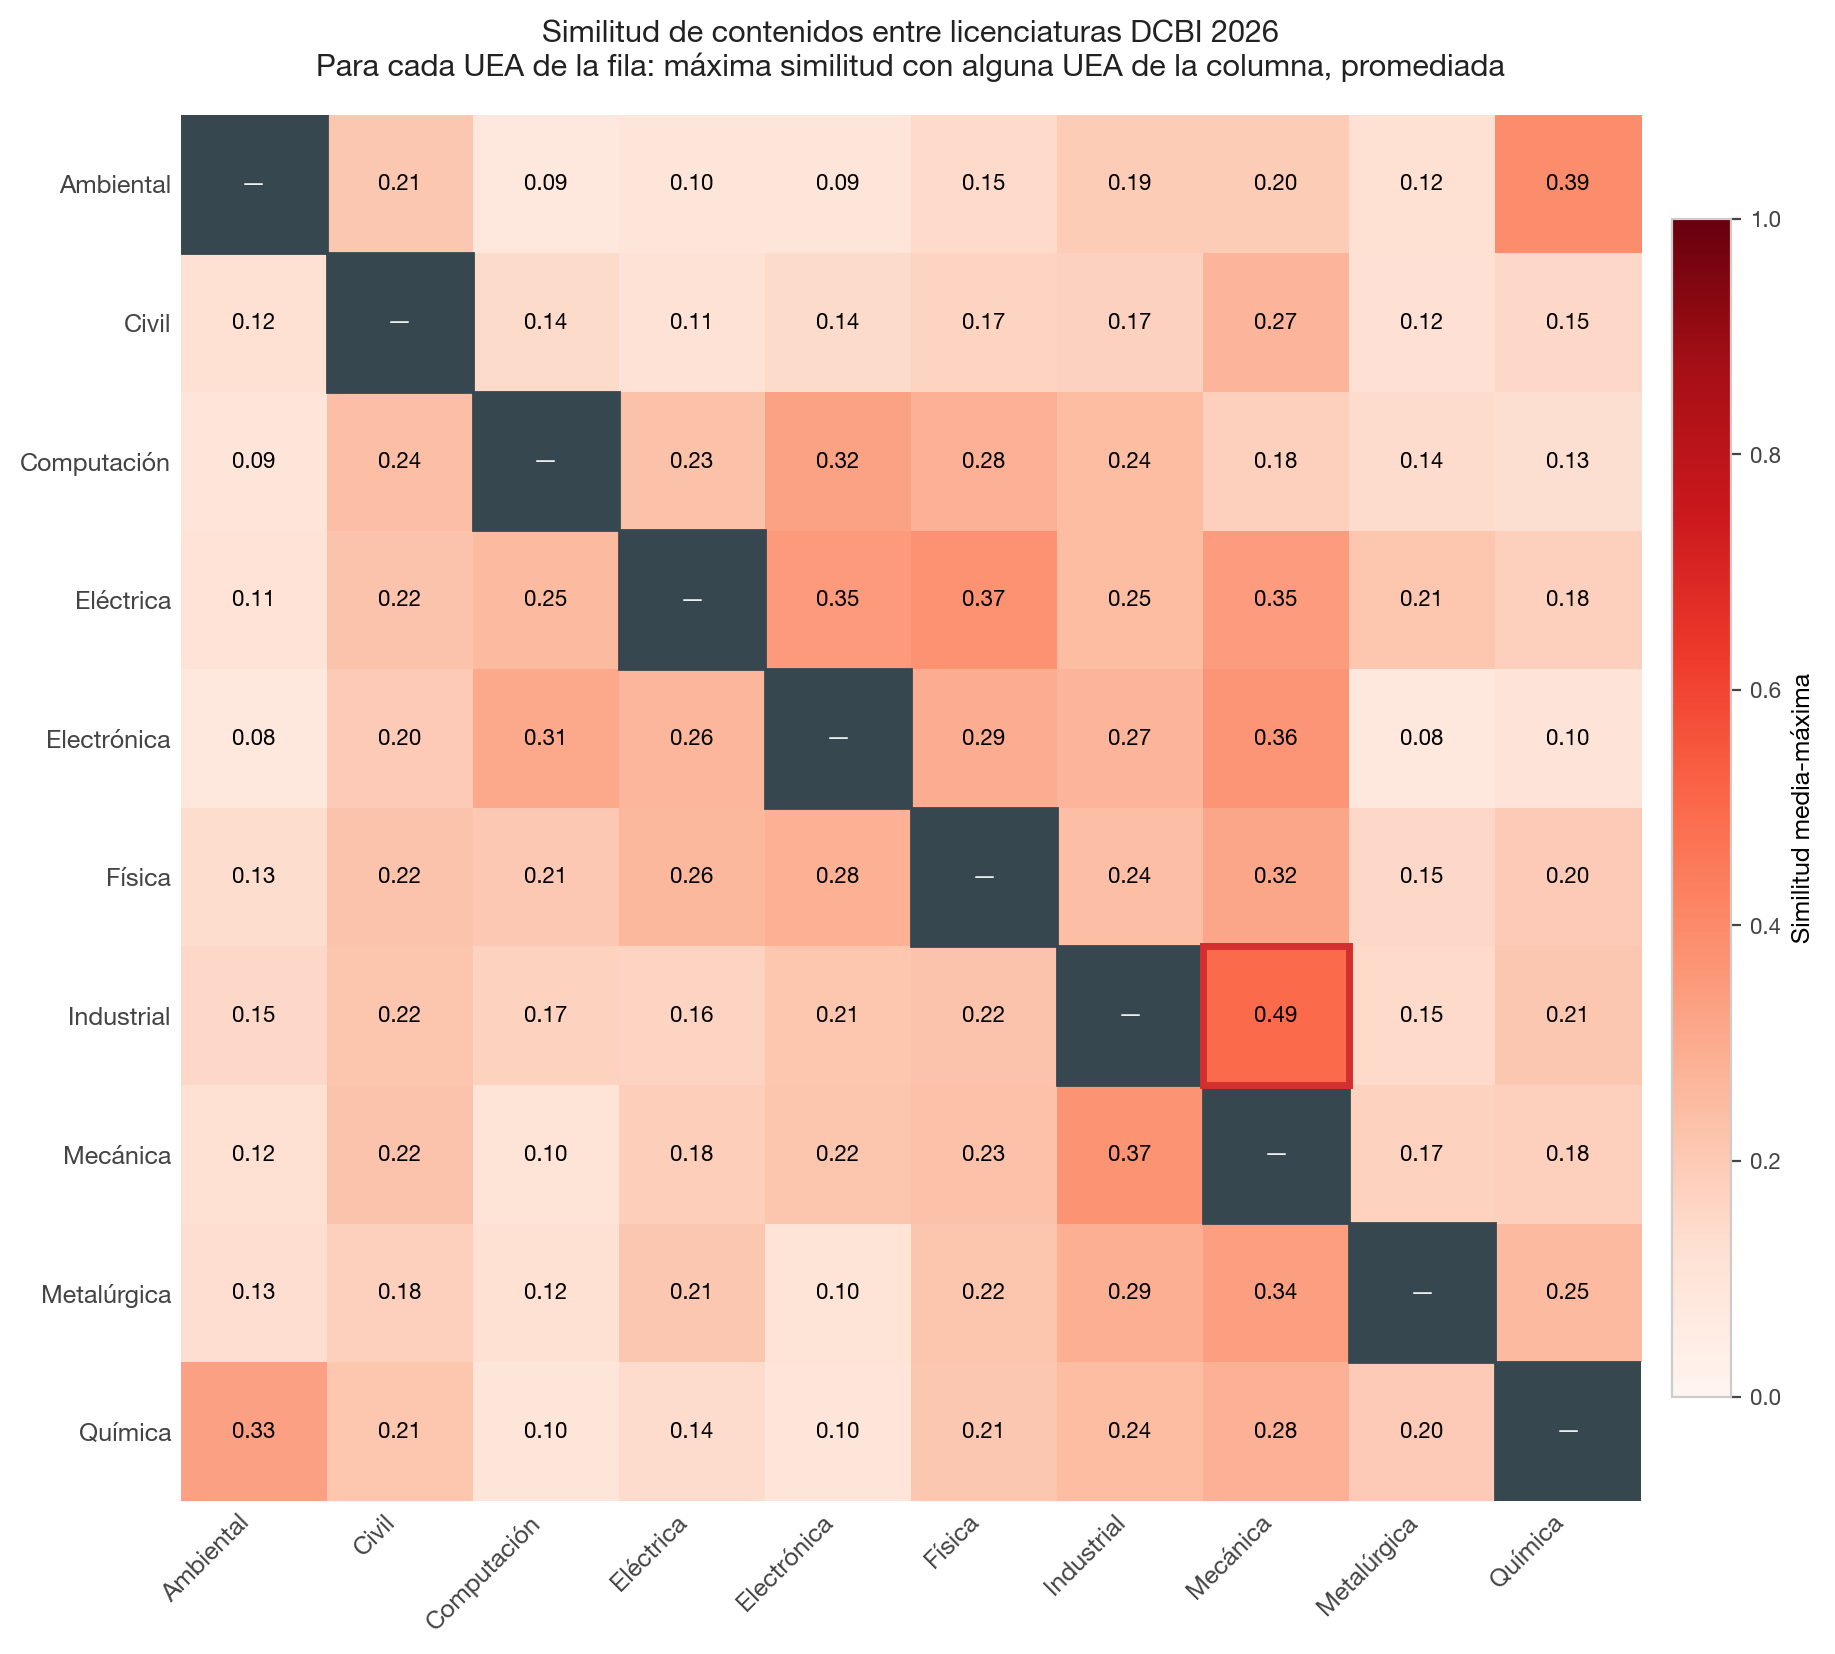
\includegraphics[width=\linewidth]{Figuras/heatmap_licenciaturas.png}
\par\vspace{1pt}
{\tiny\color{uamgray}Celda $(A,B)$: fracción del contenido de $B$ cubierta por los programas de $A$.
Escala: amarillo = baja similitud; rojo = alta similitud. Diagonal = 1 (auto-similitud).}
\end{tcolorbox}
\end{minipage}\hfill
\begin{minipage}[t]{0.413\linewidth}
\SECTHEAD{resultados de la matriz híbrida}
\begin{tcolorbox}[findcard,colback=uamred!7,colframe=uamred,
  borderline west={3pt}{0pt}{uamred}]
\MEDNUM{\color{uamred}391}\;{\LABEL{pares inter-plan}}\\
\NOTE{con $s \geq 0.30$ entre licenciaturas distintas}
\end{tcolorbox}
\begin{tcolorbox}[findcard,colback=navy!7,colframe=navy,
  borderline west={3pt}{0pt}{navy}]
\MEDNUM{\color{navy}217}\;{\LABEL{pares intra-plan}}\\
\NOTE{con $s \geq 0.40$ dentro del mismo plan}
\end{tcolorbox}
\begin{tcolorbox}[findcard,colback=teal!7,colframe=teal,
  borderline west={3pt}{0pt}{teal}]
\MEDNUM{\color{teal}455}\;{\LABEL{pares nuevos por LLM}}\\
\NOTE{detectados semánticamente ($s_{\mathrm{TF\text{-}IDF}}<0.40$)}
\end{tcolorbox}
\vspace{4pt}
\begin{tcolorbox}[enhanced,colback=forest!9,colframe=forest!35,
  sharp corners,left=7pt,right=7pt,top=5pt,bottom=5pt]
\centering
\MEDNUM{\color{forest}+154\,\%}\;{\small\color{uamblue}pares inter-plan}\\[-1pt]
{\NOTE{vs.\ TF-IDF solo}}\\[3pt]
\MEDNUM{\color{forest}+75\,\%}\;{\small\color{uamblue}pares intra-plan}\\[-1pt]
{\NOTE{vs.\ TF-IDF solo}}
\end{tcolorbox}
\end{minipage}

\vspace{3pt}

%% ── Heatmap de conteo entre pares de licenciaturas + extremos ──────────────
\begin{minipage}[t]{0.572\linewidth}
\begin{tcolorbox}[figbox]
{\footnotesize\bfseries\color{uamblue}Número de UEAs equivalentes entre cada par de licenciaturas ($s\geq0.70$)}\par\vspace{2pt}
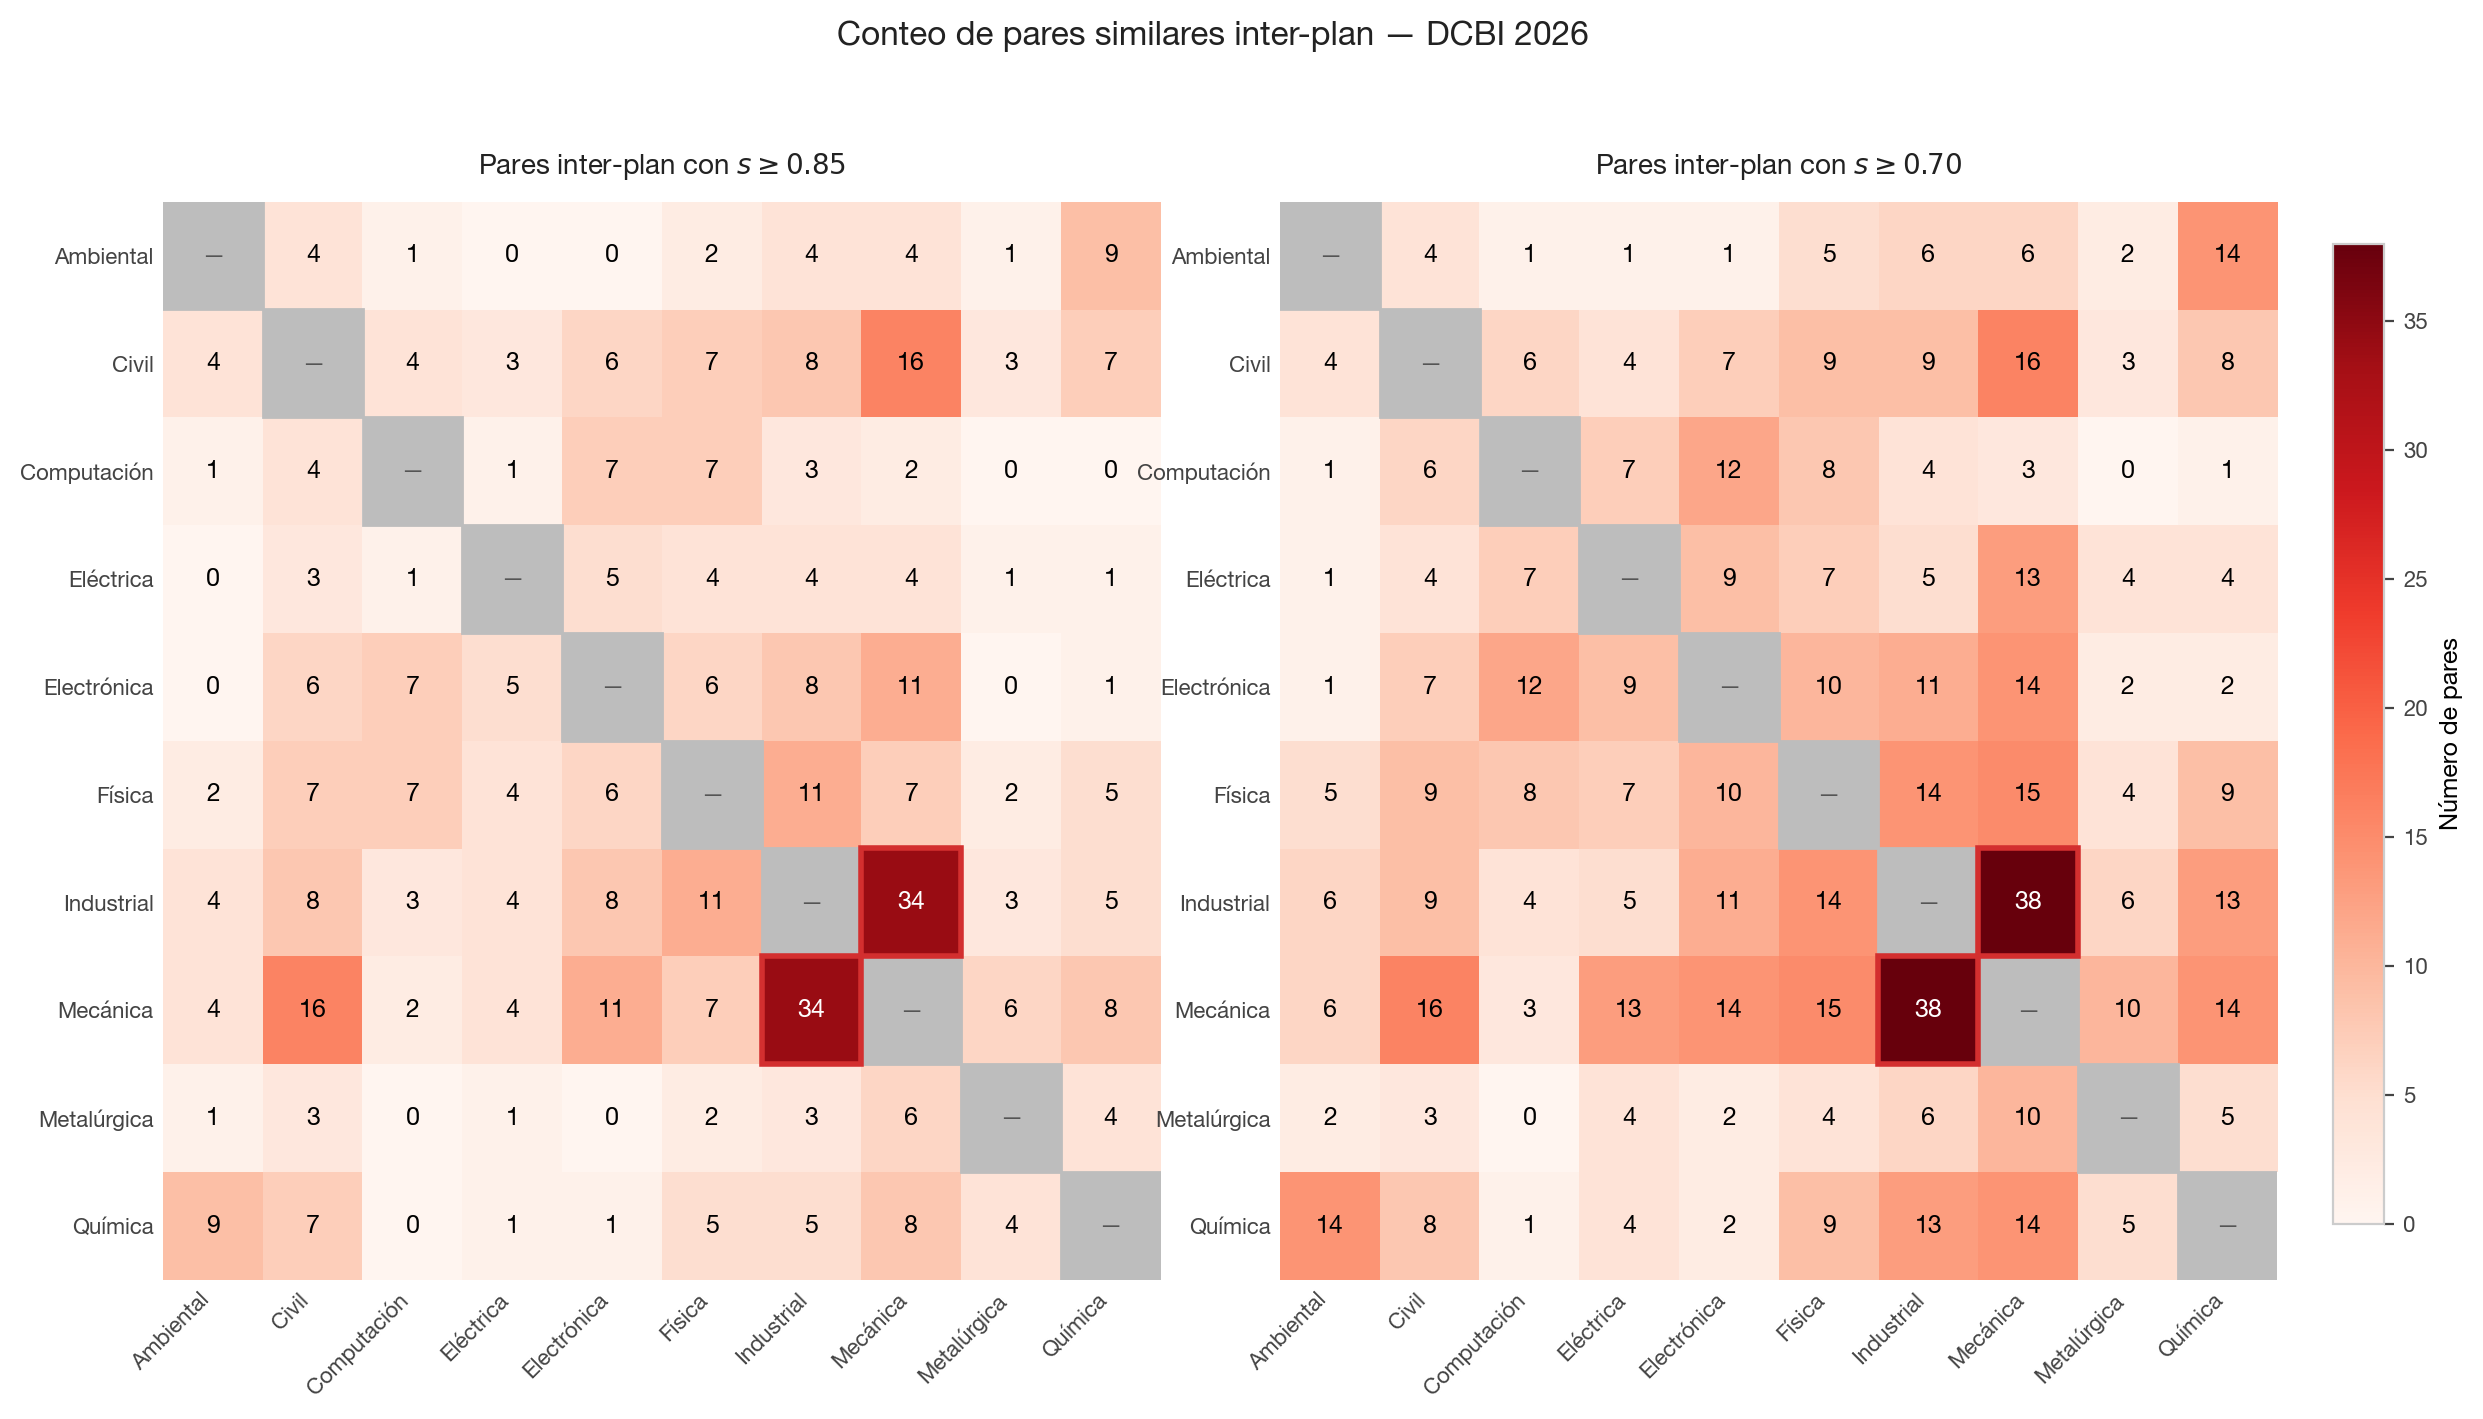
\includegraphics[width=\linewidth]{Figuras/heatmap_interplan_conteo.png}
\par\vspace{1pt}
{\tiny\color{uamgray}%
Panel izq.: umbral $s\geq0.85$ (equivalencia muy alta).
Panel der.: $s\geq0.70$ (equivalencia alta o mayor).
Par dominante: Industrial--Mecánica con \textbf{38 UEAs}.}
\end{tcolorbox}
\end{minipage}\hfill
\begin{minipage}[t]{0.396\linewidth}
\SECTHEAD{extremos del corpus}
\begin{tcolorbox}[findcard,colback=cInd!7,colframe=cInd,
  borderline west={3pt}{0pt}{cInd}]
{\small\bfseries\color{cInd}Par de mayor traslape}\\
{\small\color{uamblue}Industrial -- Mecánica}\\
\MEDNUM{\color{cInd}38}\;\NOTE{UEAs a $s\geq0.70$}\\
\MEDNUM{\color{cInd}34}\;\NOTE{UEAs a $s\geq0.85$}
\end{tcolorbox}
\begin{tcolorbox}[findcard,colback=cCiv!7,colframe=cCiv,
  borderline west={3pt}{0pt}{cCiv}]
{\small\bfseries\color{cCiv}Segundo y tercer par}\\
{\small\color{uamblue}Civil--Mecánica:\;\textbf{16}\,\NOTE{UEAs}}\\
{\small\color{uamblue}Ambiental--Química:\;\textbf{14}\,\NOTE{UEAs}}
\end{tcolorbox}
\begin{tcolorbox}[findcard,colback=cMet!7,colframe=cMet,
  borderline west={3pt}{0pt}{cMet}]
{\small\bfseries\color{cMet}Par sin traslape}\\
{\small\color{uamblue}Computación -- Metalúrgica}\\
\MEDNUM{\color{cMet}0}\;\NOTE{UEAs a $s\geq0.70$}
\end{tcolorbox}
\end{minipage}

\newpage

%%════════════════════════════════════════════════════════════════════════════
%% PÁGINA 2 — Hallazgos principales
%%════════════════════════════════════════════════════════════════════════════

%% ── Encabezado ─────────────────────────────────────────────────────────────
\begin{tcolorbox}[hdr]
{\fontsize{12.5}{14.5}\selectfont\bfseries\color{white}HALLAZGOS PRINCIPALES}\\[1pt]
{\small\color{white!70!uamred}%
Análisis de similitud · DCBI 2026 ·
Matriz híbrida TF-IDF + LLM · 626 programas de UEA}
\end{tcolorbox}

\vfill

%% ── Red de traslape + hallazgos H1–H4 ─────────────────────────────────────
\SECTHEAD{hallazgos inter-plan}
\begin{minipage}[t]{0.640\linewidth}
\begin{tcolorbox}[figbox]
{\footnotesize\bfseries\color{uamblue}Red de traslape entre licenciaturas ($s\geq0.70$, $\geq$5 UEAs)}\par\vspace{2pt}
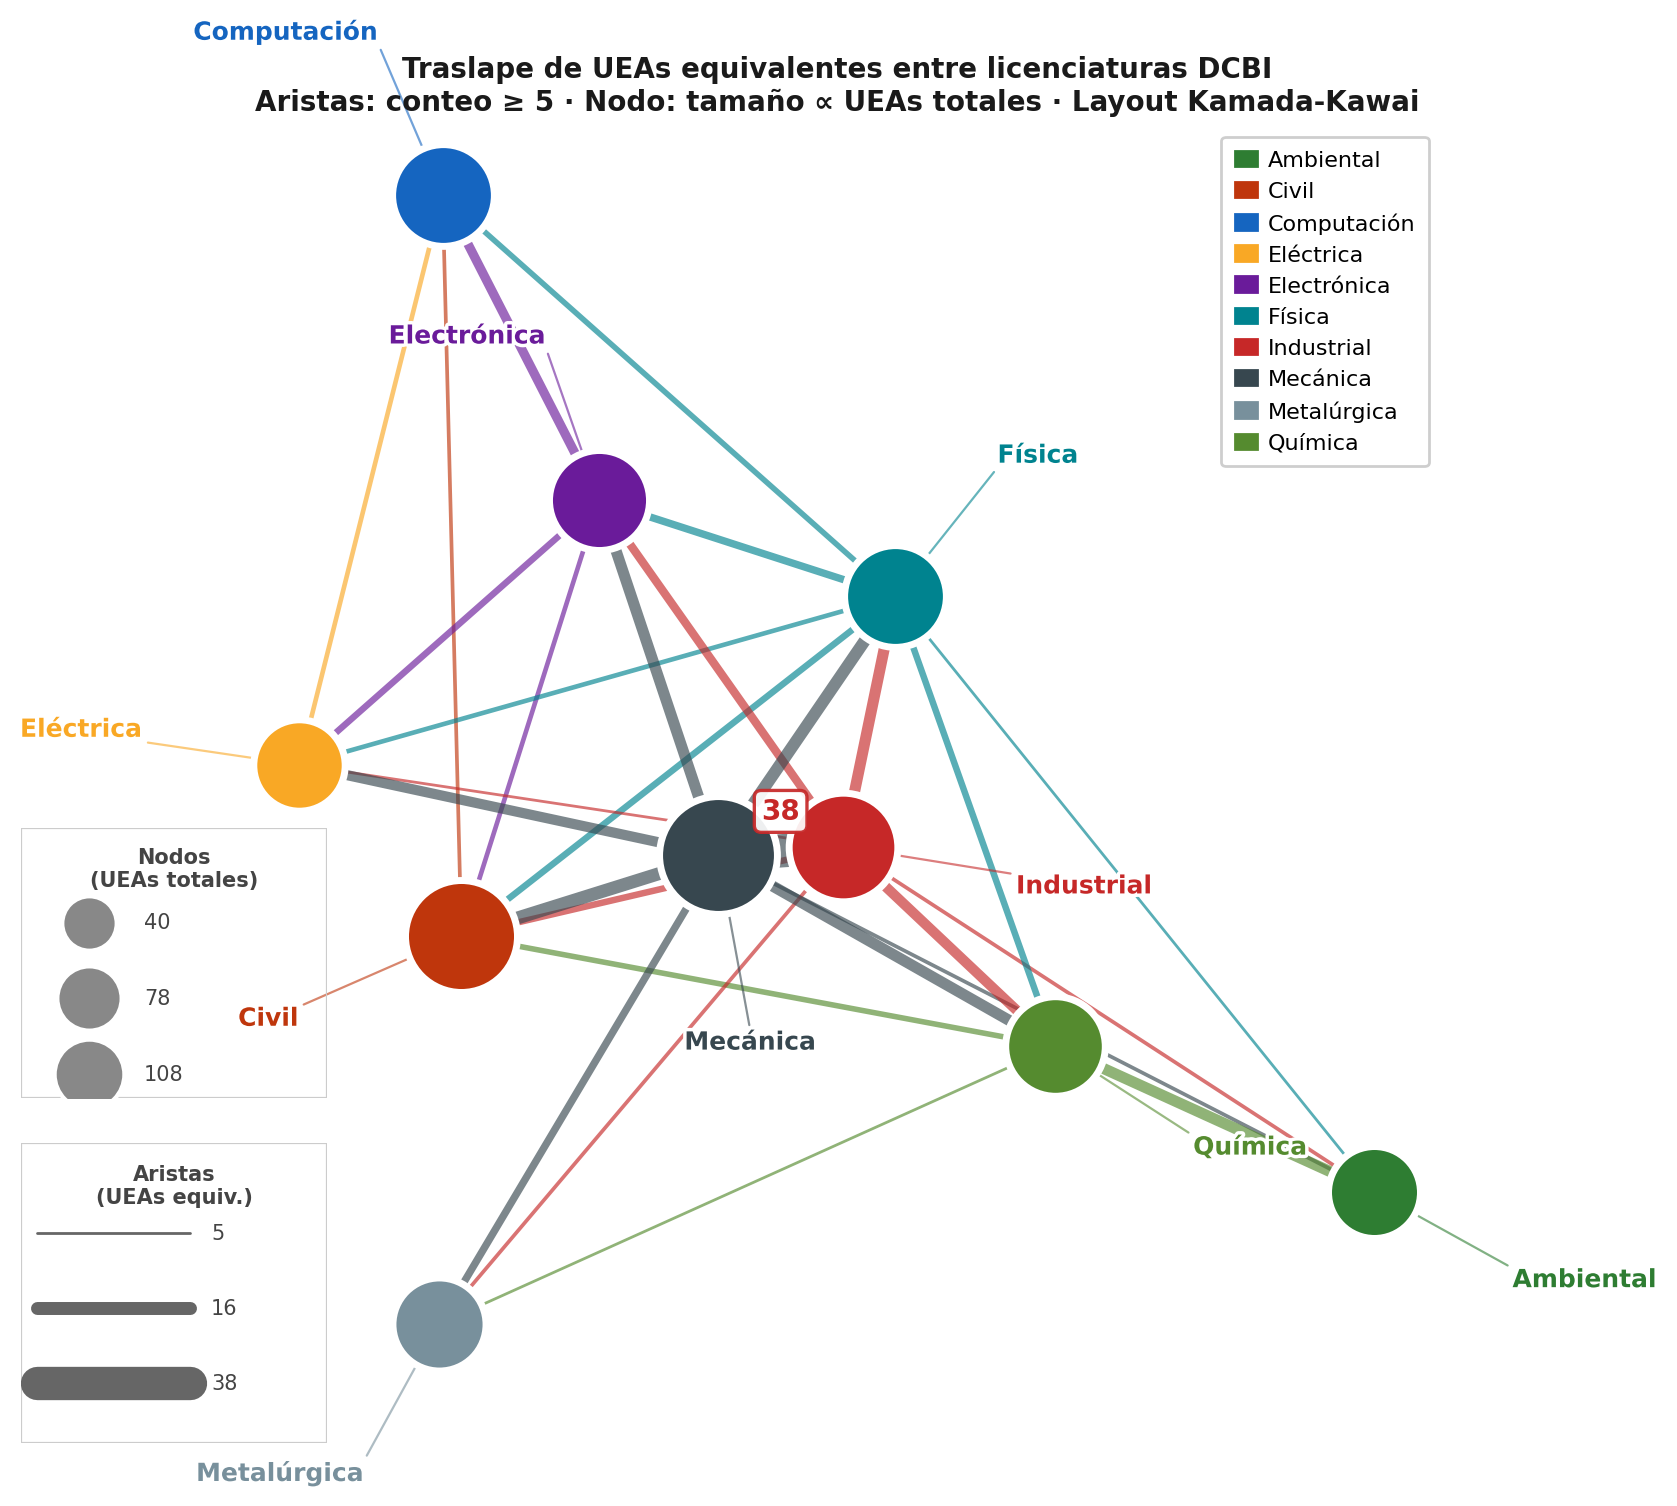
\includegraphics[width=\linewidth]{Figuras/grafo_licenciaturas_variante_B.png}
\par\vspace{1pt}
{\tiny\color{uamgray}Aristas: pares con $\geq$5 UEAs equivalentes a $s\geq0.70$ (29 de 45 pares posibles).
Grosor proporcional al conteo. Layout: Kamada-Kawai.}
\end{tcolorbox}
\end{minipage}\hfill
\begin{minipage}[t]{0.335\linewidth}
\begin{tcolorbox}[findcard,colback=cInd!6,colframe=cInd,
  borderline west={4pt}{0pt}{cInd}]
{\small\bfseries\color{cInd}H1 · Industrial -- Mecánica}\\[2pt]
\BIGNUM{\color{cInd}38}\;\LABEL{UEAs a $s\geq0.70$}\\
\NOTE{34 a $s\geq0.85$ $\cdot$ manufactura, materiales,
termodinámica, métodos numéricos}
\end{tcolorbox}
\begin{tcolorbox}[findcard,colback=cFis!6,colframe=cFis,
  borderline west={4pt}{0pt}{cFis}]
{\small\bfseries\color{cFis}H2 · Física — nodo transversal}\\[2pt]
\BIGNUM{\color{cFis}100}\;\LABEL{pares inter-plan}\\
\NOTE{Conectada con las 10 licenciaturas.
Mayor conectividad del corpus.}
\end{tcolorbox}
\begin{tcolorbox}[findcard,colback=cAmb!6,colframe=cAmb,
  borderline west={4pt}{0pt}{cAmb}]
{\small\bfseries\color{cAmb}H4 · Ambiental -- Química}\\[2pt]
\BIGNUM{\color{cAmb}14}\;\LABEL{UEAs a $s\geq0.70$}\\
\NOTE{9 a $s\geq0.85$ · núcleo de ingeniería
ambiental implícito en ambos planes.}
\end{tcolorbox}
\begin{tcolorbox}[findcard,colback=uamlgray,colframe=uamlgray,
  borderline west={4pt}{0pt}{uamgray}]
{\small\bfseries\color{uamblue}H3 · Bloque de ing.\ clásicas}\\
\NOTE{Mecánica, Industrial, Física y Electrónica: $\geq$10 UEAs entre cada par.
Civil se acopla a Mecánica con 16 UEAs equivalentes.}
\end{tcolorbox}
\end{minipage}

\vfill

%% ── Contenidos transversales de facto (H5–H8) ──────────────────────────────
\begin{tcolorbox}[grayband]
\SECTHEAD{h5–h8 · contenidos transversales de facto — sin coordinación formal entre licenciaturas}
\begin{minipage}[t]{0.237\linewidth}
\begin{tcolorbox}[famcard,colback=navy!10,colframe=navy]
\centering
{\footnotesize\bfseries\color{navy}Ecuaciones Diferenciales}\\[2pt]
\MEDNUM{\color{navy}9\,/\,10}\;{\footnotesize\color{uamblue}planes}\\
{\tiny $s=1.00$ · claves distintas}\\[1pt]
{\tiny\color{uamgray}Contenido idéntico en 9 planes; cada licenciatura
registra su propia UEA con clave distinta.}
\end{tcolorbox}
\end{minipage}\hfill
\begin{minipage}[t]{0.237\linewidth}
\begin{tcolorbox}[famcard,colback=amber!15,colframe=amber]
\centering
{\footnotesize\bfseries\color{amber}Liderazgo y Emprendimiento}\\[2pt]
\MEDNUM{\color{amber}9\,/\,10}\;{\footnotesize\color{uamblue}planes}\\
{\tiny $s_{\mathrm{LLM}}\geq0.72$}\\[1pt]
{\tiny\color{uamgray}Invisible a TF-IDF ($s\approx0.22$). Solo
detectable mediante re-evaluación semántica.}
\end{tcolorbox}
\end{minipage}\hfill
\begin{minipage}[t]{0.237\linewidth}
\begin{tcolorbox}[famcard,colback=cAmb!10,colframe=cAmb]
\centering
{\footnotesize\bfseries\color{cAmb}Ed.\ Ambiental y\\Cambio Climático}\\[2pt]
\MEDNUM{\color{cAmb}$\geq$6}\;{\footnotesize\color{uamblue}planes}\\
{\tiny $s\geq0.95$}\\[1pt]
{\tiny\color{uamgray}Civil, Eléctrica, Electrónica,
Física, Mecánica, Química: contenido convergente.}
\end{tcolorbox}
\end{minipage}\hfill
\begin{minipage}[t]{0.237\linewidth}
\begin{tcolorbox}[famcard,colback=teal!10,colframe=teal]
\centering
{\footnotesize\bfseries\color{teal}Núcleo matemático\\(4 UEAs)}\\[2pt]
\MEDNUM{\color{teal}5}\;{\footnotesize\color{uamblue}planes c/u}\\
{\tiny $s\geq0.98$}\\[1pt]
{\tiny\color{uamgray}Cálculo Integral · Prob.\ y Est.\ Descriptiva ·
Métodos Numéricos · Prog.\ Aplic.\ a la Ing.}
\end{tcolorbox}
\end{minipage}
\end{tcolorbox}

\vfill

%% ── Análisis intra-plan (H10–H14) ──────────────────────────────────────────
\begin{tcolorbox}[whitebox]
\SECTHEAD{h10–h14 · hallazgos intra-plan}
\begin{minipage}[t]{0.237\linewidth}
\begin{tcolorbox}[famcard,colback=uamred!7,colframe=uamred,
  borderline west={3pt}{0pt}{uamred}]
{\footnotesize\bfseries\color{uamred}3 duplicados documentales}\\[1pt]
{\tiny\color{uamgray}%
\textcolor{cQui}{$\bullet$}~Química: Análisis de Ciclo de Vida ($s=0.990$)\\
\textcolor{cFis}{$\bullet$}~Física: Aplic.\ Exp.\ I y II ($s=0.950$)\\
\textcolor{cInd}{$\bullet$}~Industrial: clave 1100202 duplicada}
\end{tcolorbox}
\end{minipage}\hfill
\begin{minipage}[t]{0.237\linewidth}
\begin{tcolorbox}[famcard,colback=cCiv!7,colframe=cCiv,
  borderline west={3pt}{0pt}{cCiv}]
{\footnotesize\bfseries\color{cCiv}Civil: 61 pares ($s\geq0.40$)}\\[1pt]
{\tiny\color{uamgray}Mayor densidad intra-plan del corpus.
TF-IDF detectaba solo 8.
Objetivos convergentes: estructuras, hidráulica, geotecnia.}
\end{tcolorbox}
\end{minipage}\hfill
\begin{minipage}[t]{0.237\linewidth}
\begin{tcolorbox}[famcard,colback=cCmp!7,colframe=cCmp,
  borderline west={3pt}{0pt}{cCmp}]
{\footnotesize\bfseries\color{cCmp}Computación: 24 falsos positivos}\\[1pt]
{\tiny\color{uamgray}TF-IDF: 57 pares → LLM confirmó 33
y descartó 24. Vocabulario genérico de software
elevaba artificialmente la similitud.}
\end{tcolorbox}
\end{minipage}\hfill
\begin{minipage}[t]{0.237\linewidth}
\begin{tcolorbox}[famcard,colback=cMet!7,colframe=cMet,
  borderline west={3pt}{0pt}{cMet}]
{\footnotesize\bfseries\color{cMet}Metalúrgica: 3 → 29 pares}\\[1pt]
{\tiny\color{uamgray}Mayor incremento relativo.
Vocabulario técnico heterogéneo entre versiones
de una misma UEA. Pares taller/teoría.}
\end{tcolorbox}
\end{minipage}
\end{tcolorbox}

\vfill

%% ── URL / pie ─────────────────────────────────────────────────────────────
\begin{tcolorbox}[enhanced,colback=uamred!5,colframe=uamlgray,
  sharp corners,left=6pt,right=6pt,top=3pt,bottom=3pt]
\centering
{\footnotesize\color{uamgray}Figuras interactivas y datos completos:}\quad
{\footnotesize\bfseries\color{uamred}\texttt{cslmuam.github.io/similitud-dcbi-2026}}
\end{tcolorbox}

\end{document}
